\section{ARCHITECTURAL DESIGN}



\subsection{Architectural Diagram}

\begin{figure}[H]
\centering
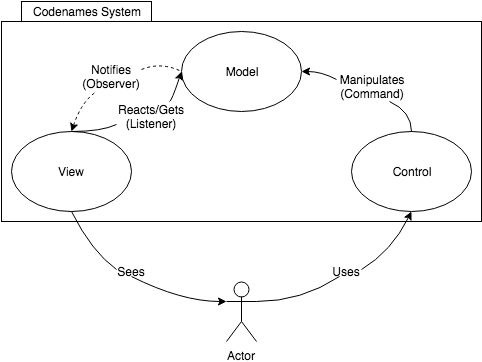
\includegraphics[width=10cm]{Source/MVC.png}
\caption{System Architecture based on Model-View-Control design}
\label{View}
\end{figure}

%A UML class diagram or package diagram depicting the high-level structure of the system,
%accompanied by a one-paragraph text describing the rationale of this design.
%It is mandatory that the system be divided into at least two subsystems,
%and that the purpose of each of these subsystems be exposed here.

%==============

The Codenames game project specifications call for a graphical interface that can reflect an evolving game state and a system through which user input is processed to alter the game state. The application is a layered logical architecture composed of three subsystems inspired and named after the Model-View-Controller (MVC) separation principle. This principle provides a logical approach to dividing the domain, user interface, and application layers into subsystems that can be developed independently and, through interfaces, interact with each other. This section provides a description of the responsibility of each subsystem and discusses the reasoning behind choosing to model this systems architecture according to MVC. \\

The Model subsystem represents the current game state through its three component packages: Board, which represents the data relating to the ongoing game, Player, which represents the players and their strategies (using the Strategy pattern), and Util, which logs everything that takes place in Model. In general, the Model subsystem is synonymous to the domain layer, and is therefore an inspirational creation of the domain model. \\

The View subsystem contains all objects that provide a user-friendly interface to the Codenames game. These objects are responsible for capturing input, and output. They may sometimes produce graphical elements. However, they are not responsible for containing data pertaining to the state of the game, nor do they incorporate any logical behaviour affecting the internals of the application. In the Codenames application, the View subsystem uses the Observer pattern to bind itself to specific Subject classes in the Model subsystem to display the current game state in real time. This allows the Model subsystem to function uninterrupted, independently of the View subsystem. \\

The Control subsystem contains all objects tasked with defining the stimulus and/or handling stimuli forwarded by the View subsystem. In this context, a stimulus is defined as a request, or message that initiates work to be performed by the system. Furthermore, objects in this subsystem possess functional characteristics. In the Codenames application, the game progresses through one turn when the user presses the "Enter" key. The action of a user pressing “Enter” is handled by the GameHandler, which through the Command design pattern, commands the Model classes to do the next turn, changing the Models state, and updating the View accordingly. \\

\subsection{Subsystem Interface Specifications}
In general, the Model and View  according to the Observer design pattern, and the Controller controls the Model by making commands through the Command design pattern. This section specifies the actual function calls which make up these software interfaces between the three (MVC) subsystems. Outside of the two design patterns defined about, most of the Model's interface is functions called by View classes to get the internal state of the game, on which the GUI is based.

\subsubsection {Model Subsystem Interface}
The communication between the Model and View subsystems is implemented in the Observer Design Pattern. As a result, the Model contains classes which extend the Subject abstract class, to which Observer classes in the View may attach() themselves, so that they are notified to changes in the Subject's state. The GameManager, Verbose, and Card classes are Subjects.

\textbf{Subject} An abstract class for Subject's in the Observer design pattern.
\begin{itemize}
  \item void attach(Observer o): add the Observer object o to the list of Observers to be notified upon changes of state.
  \item String getStringProperty(): returns the Subject's state in the form of a String.
  \item CardType getTypeProperty(): returns the Subject's state in the form of a CardType (Red, Blue, Assassin, Bystander).
\end{itemize}

\textbf{GameManager} The GameManager class keeps track of much of the state of the game. It is a Subject, serving as an interface for the View to get data on the games state. Along with the methods of Subject, the GameManager class has the following methods:
\begin{itemize}
  \item void doNextTurn(): The main interface between the Controller and the Model. This initiates the Model to do the next turn, changing the state of the game.
  \item Clue getCurrentClue(): Returns the Clue given by the current team.
  \item int getBlueScore(): Returns the number of cards left for Blue to guess.
  \item int getRedScore(): Returns the number of cards left for Red to guess.
  \item CardType getWinner(): Returns void if nobody has yet won, or CardType.Blue, or CardType.Red if there has been a winner.
\end{itemize}

\textbf{CardBuilder} The CardBuilder class is a helper class for extracting the word data from the .txt files, and turning it into a randomized board. It is used to start a game.
\begin{itemize}
  \item Card[] buildAll(): Returns 25 Cards, generated from the database of nouns and keycards. Used to initialize the game.
\end{itemize}

\textbf{Verbose} The Verbose class is used for logging in the Model. It is a Subject. It uses the Subject's getStringProperty() method to notify its Observers of log messages. It is a Singleton, and as a result has the following methods:
\begin{itemize}
  \item get() Returns the one instance of Verbose.
  \item bind(Observer) attaches Observers to the instance of Verbose.
\end{itemize}

\subsubsection {View Subsystem}
The View subsystem will start by calling start(Stage) that will create a new verboseView and Verbose object.
Codenames class is also responsible for building the GameScene this class calls build(Subject[], Event\textless KeyEvent\textgreater ) of type scene that will set up user input to send to the CardPane class. After GameScene create a CardPane object, it will hold the images of the cards and where each card is place on the board to display. The Verbose object will call bind(Observer) to bind an Observer object to the game board to record events. log(String) will capture events and convert them to phrases that will display in VerboseView. Lastly, a Subject object can call attach(Observer) to attach a new Observer to it which will keep track of things in the Model subsystem.

\textbf{CardPane} A class that implements the Observer to represent the GUI of 1 card on the board. It is covered until the update function is called.
\begin{itemize}
  \item update() Called by subject of class to reveal color of card with image.
\end{itemize}

\subsubsection {Control Subsystem}
The control subsystem creates the command package. Codename's start(Stage) will create a new GameHandler object. This will contain information about the model's GameManager, the View's score and verbose and the control's commandManager and store a history of used commands. The handle(KeyEvent) will control the action on which key is pressed to execute the appropriate command and change the state of the game in the model. After GameHandler, creates a CommandManager, it will be able to create and execute() Command objects. GameHandler also makes a NextTurnCommand object that controls the turn flow of the game to set the input to match the game's commands.\\

The Difficulty class sets the different strategies that each player type will be able to use. Using setDifficulty(), the user is able to select their difficulty and use the appropriate strategy that is stored in the model subsystem. 

\textbf{GameControls} A class responsible for handling the events of restarting or quitting the game. The game board will be reset upon restarting the game or will terminate upon selecting quit.
\begin{itemize}
  \item setEvents() Sets the menu items and actions for the game which includes (Restart) and (Quit).
  \item setAbout() Sets the description of the menu items in a new window.
\end{itemize}



\newpage
